\section{Background}
\vspace{-0.5cm}
\subsection{Microneedles as Biosensors}
\vspace{-0.5cm}
Microneedle-based diagnostic platforms can be divided into three main categories: biofluid extraction involving direct extraction of skin ISF with hollow and hydrogel MNs, specific target analyte capture and electrochemical biosensing with solid and hollow MNs acting as an electrode base for further modification \cite{dixon2021microneedle}. For continuous monitoring, MNs need to be coupled with electrochemical electrodes. These electrochemical MN biosensors consist of a signal transducer (the MN) coated with a recognition element (nucleic acid aptamers, etc.) that forms specific interactions with the target biomarker, transmitting a quantifiable electrical signal that correlates with the target’s concentration.
\begin{center}
    \begin{figure}[H]
    \centering
    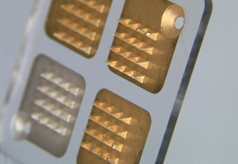
\includegraphics[width=.4\textwidth]{img/microneedle_patch.png}
    \caption{Example Image of a Microneedle array for for real-time, minimally invasive drug monitoring of phenoxymethylpenicillin \cite{rawson2019microneedle}}
    \label{fig:microneedle}
\end{figure}
\end{center}
\vspace{-1cm}
% Signal quantifying techniques include amperometry, voltammetry, potentiometry and impedance spectrometry. Voltammetric or amperometric sensors measure current changes caused by redox reactions. Potentiometric sensors measure changes in potential caused by local ion flux from target interactions. Impedance-based biosensors measure changes in resistance at the electrode surface using alternating currents.\\\\
Our MN has two main application purposes: (1) access the ISF by penetrating the skin barrier and (2) act as a platform for the recognition element. Hence, more holistic research has been performed on skin structure and MN device considerations, detailed in Appendix Part A.
\subsection{Nitrite Investigations}
Nitrite has been found to be a more sensitive and specific biomarker for the diagnosing septic shock compared  to known biomarkers such as procalcitonin (PCT), C-reactive protein (CRP) and interleukin-6 (IL-6), and its concentration remains elevated days after admission \cite{pmid9142024}.\\\\
We aim to measure nitrite concentration in solution by performing a differential pulse voltammagram, followed by obtaining a calibration curve, examining the reduction of nitrite (NO$^{2-}$) to nitrate(NO$^{3-}$). This reaction is shown in \autoref{eqn:nitriteredox1} and \autoref{eqn:nitriteredox2}.
\begin{align} \label{eqn:nitriteredox1}
   NO\textsubscript{2}\textsuperscript{-} \ \xrightleftharpoons{}  NO\textsubscript{2} \ + \  e\textsuperscript{-}
\end{align} 
\begin{align}\label{eqn:nitriteredox2}
  2NO\textsubscript{2} \ + \ H\textsubscript{2}O \xrightarrow{}\  2H\textsuperscript{+} \ + \ NO\textsubscript{2}\textsuperscript{-} \ + \  NO\textsubscript{3}\textsuperscript{-}
\end{align}
Differential pulse voltammetry (DPV) measures the concentration of electrolytes in solution by applying potential (E) at the working electrode (WE) and reference electrode (RE). A series of pulses of increasing steps is applied to the WE and the difference in current between steps is measured \cite{D1CP00661D}. A calibration curve is then constructed from the peaks of the curve using linear regression. \\\\
Experiments utilising disposable gold electrodes, where the WE, RE and CE are all located on a 10mm x 8mm polycarbonate surface were then performed. These electrodes have been shown to have good electrochemical response, as well as being cheap and disposable, favouring use in a clinical setting as a biosensor \cite{FERRARIO201236}.\\\\
Albumin is found in human blood in the range of 33–52 g/L. There is some evidence that presence of albumin may interfere with electrode activity, which may be due to precipitate forming on the electrode surface, thus reducing surface area \cite{doi:10.1177/000456329102800111}.
%======================================================================================================
\subsection{Hydrogen Peroxide Investigations}
Hydrogen peroxide, H\textsubscript{2}O\textsubscript{2}, is a chemical that is commonly found in multiple biological processes. It is found that the presence of hydrogen peroxide in human blood serum and interstitial fluid is usually accompanied with infections. Moreover, the \textit{in vivo} concentration of hydrogen peroxide shows a strong correlations with the severity of the infection. From previous literature research, hydrogen peroxide presents a high sensitivity and specificity, specifically with respect to sepsis - a critical clinical sign of infection. Therefore, hydrogen peroxide serves as one of the novel biomarkers that demonstrates a high suitability for clinical continuous-monitoring techniques using microneedles.  Its outstanding capability in identifying sepsis and indicating the severity of infection provides a high significance in sepsis diagnosis, evolution evaluation and prognosis prediction.\\\\
\noindent To sensing the presence of hydrogen peroxide, a strategy based on the reduction-oxidation (redox) reactions between hydrogen peroxide and Prussian blue (PB) is proposed by Chen \textit{et al} \cite{C9AN02438G}. Prussian blue, also known as ferric ferrocyanide, is an artificially synthesised chemical complex that demonstrates an outstanding hydrogen peroxide sensing range with low operating potential. This two-step reaction commences by reducing Prussian blue to Prussian white (PW), as shown in \autoref{eqn:h2o2redox1}. Following the first step, Hydrogen peroxide is further reduced to water, as shown in \autoref{eqn:h2o2redox2}.
\begin{align} \label{eqn:h2o2redox1}
    KFe^{3+}[Fe\textsuperscript{2+}(CN)\textsubscript{6}]\textsuperscript{4-} \ + \ & K\textsuperscript{+} \ + \   e\textsuperscript{-} \ \xrightleftharpoons{} \\ \nonumber & K\textsubscript{2}Fe\textsuperscript{2+}[Fe\textsuperscript{2+}(CN)\textsubscript{6}]\textsuperscript{4-}
\end{align}
\begin{align} \label{eqn:h2o2redox2}
    & 2K\textsubscript{2}Fe\textsuperscript{2+}[Fe\textsuperscript{2+}(CN)\textsubscript{6}]\textsuperscript{4-} \ + \  H\textsubscript{2}O\textsubscript{2} \ + \ 2H\textsuperscript{+} \ \xrightleftharpoons{} \\ \nonumber & \quad \quad 2K\textsubscript{2}Fe\textsuperscript{3+}[Fe\textsuperscript{2+}(CN)\textsubscript{6}]\textsuperscript{4-} \ + 2H\textsubscript{2}O \ + \ 2K\textsuperscript{+}
\end{align}
\noindent A graphical visualization to the reactions between H\textsubscript{2}O\textsubscript{2} and PB can be found in \autoref{fig:pb_h2o2}.
\begin{figure}[H]
    \centering
    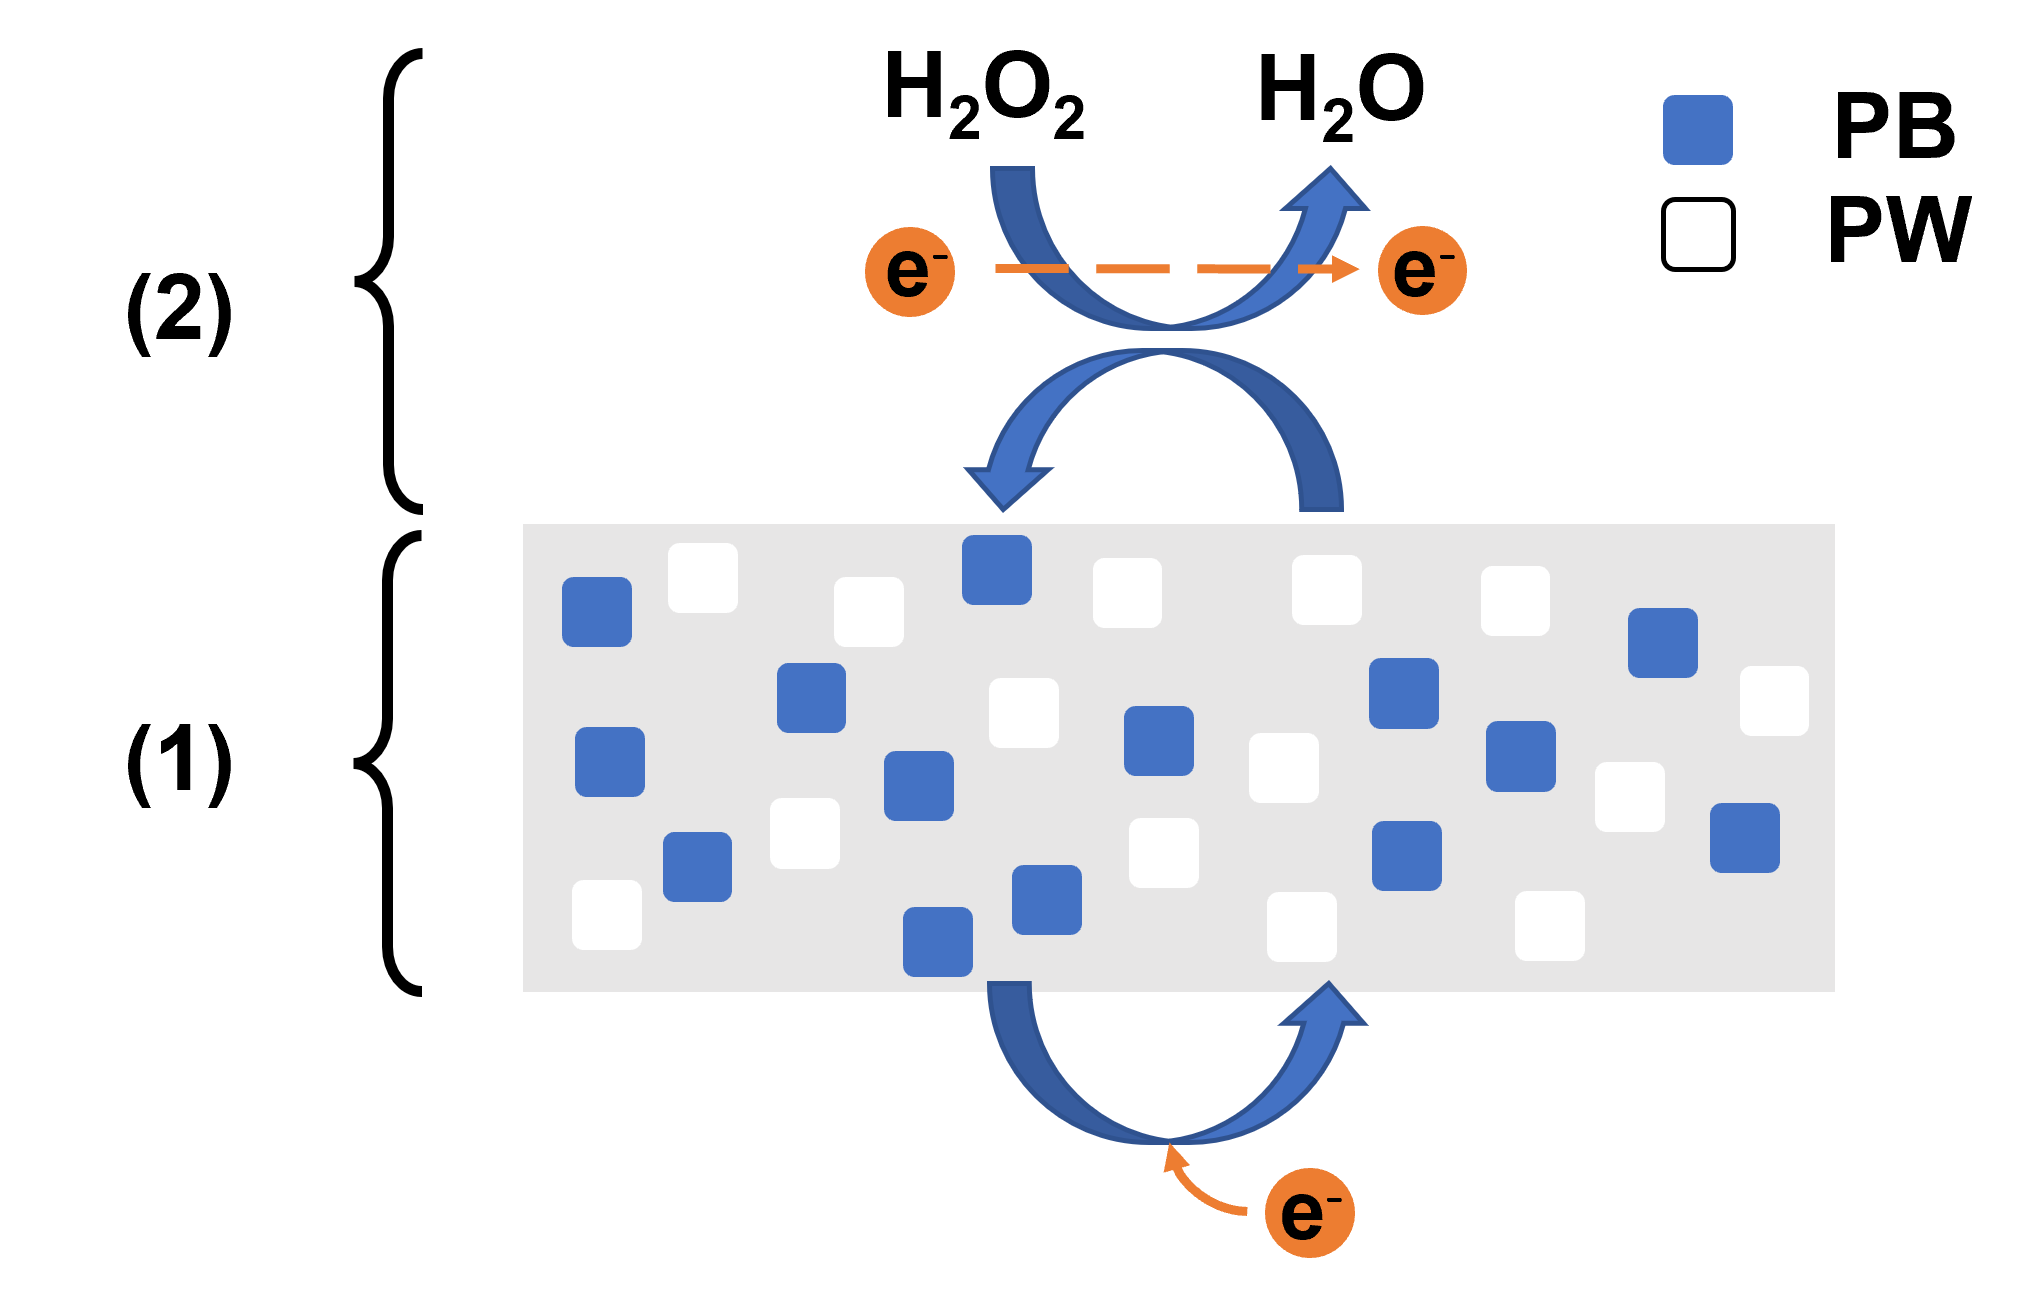
\includegraphics[width=.5\textwidth]{img/pb_h2o2.png}
    \caption{Reaction between hydrogen peroxide and Prussian blue.}
    \label{fig:pb_h2o2}
\end{figure}
%======================================================================================================

\subsection{Lactate Investigations}
Patients suffering from sepsis often develop Sepsis-Associated HyperLactatemia (SAHL). SAHL can be explained by multiple proposed theories. The least contested and most evidential blames the increase of aerobic glycolysis rates, subsequent to adrenergic stimulation, for SAHL \cite{garcia2014sepsis}.
Hyperlacatatemia can be characterised most commonly by a serum concentration exceeding 4mmol/L however different literature demands lower thresholds can also indicate a significant septic state \cite{singer2014ed}. It is therefore important live monitoring of lactate levels can occur in clinical settings such that levels which exceed those of healthy patients or sharp increases can be detected quickly enough for antibiotics or appropriate measures to be taken before the state becomes fatal \cite{gyawali2019sepsis}.
In this project we develop enzyme-based electrode sensing for lactate detection.
\subsection{Statistics of Diagnosis}
When working with different biomarkers of sepsis it is critical that readings are specific and predictive. Especially in the case of sepsis, treatment includes administration of antibiotics- if antibiotics are delivered unnecessarily it could lead to evolution of antibiotic resistance.\\\\
To evaluate the success of a biomarker at positively indicating disease the sensitivity, specificity, predictive values and diagnostic accuracies are statistics commonly used amongst clinicians to quantify the success of the diagnostic technique at mitigating false results. To calculate each of these variables, the biomarker must be assessed for both false and true positives and negatives against a pre-established gold standard diagnosis (assumed 0 false positives). Sensitivity can be described as the ratio of observed positives to all the real number of positives (true positives/true positives + false negatives), it indicates how well the biomarker picks up disease \cite{kazmierczak1999statistical}. \\\\
Specificity is given by the ratio of true negatives observed to the actual number of negative cases (true negatives/true negatives + false positives). For particular biomarkers which can be used for various disease, the specificity can be considerably lower, owing to the higher rate of false positives. The positive predictive value gives the ratio of true positives to total positives observed (true positives/ false and true positives), whereas the negative predictive value gives the ratio of true negatives to total negatives observed (true negatives/ false and true negatives).  The overall diagnostic accuracy is given by the proportion of all true results \cite{christenson2007evidence}.\\\\
For both predictive values and overall diagnostic accuracies, variations occur with prevalence of sepsis. PPV can increase dramatically with increase prevalence and so often sensitivity and specificity are more frequently used to describe efficacy of detection methods. However, these are not immune to variability- especially in the case of sepsis. Sepsis is not always binary, it may be that a patient is at risk of septic shock or approaching levels that are indicative of entering septic shock but are not septic in that moment. In such cases a ‘cut off mark’ is not always a singular number but more often a range and often these ranges are disputed and unclear in literature \cite{xia2013translational}. \\\\
Perhaps a more useful and less discriminatory way at quantifying usefulness is looking at the relationship between sensitivity and specificity by plotting receiver operating characteristics (ROC). Where there exists a range of values rather than a single cutoff value, sensitivity and specificity value pairs can be determined for different levels of biomarker concentration. By plotting 1-specificty versus sensitivity we can obtain a ROC curve. The shape of the curve (i.e asymmetry) and the area under it, can both be used in conjunction to convey diagnostic accuracy and allow clinicians to contextualise and make decisions from the results our sensors give \cite{kampfrath2013brief}. 
\subsection{Aptamer-Based Biosensors}
% Nucleic acid aptamers are short single stranded oligonucleotides sequences that will selectively bind to specific target molecules such as biomarkers, metal ions, antibiotics and more with high affinity and specificity. They are selected using SELEX. Once the nucleic acid sequence is chosen, it can be synthesised and modified with a redox-active group. Upon binding to the target, aptamers can undergo different types of conformational changes forming structural shapes such as hairpins, bulges, and G-quadruplexes  \cite{riccitelli2010computational}. This results in a change in the distance between the redox group and electrode surface which thus leads to a change in the current.\\\\
Nucleic acid aptamers exhibit many advantages as biorecognition elements in biosensing compared to other sensing molecules such as enzymes and antibodies. They are small in size, chemically stable and cost effective \cite{song2008aptamer}. Aptamers can be isolated from a library of sequences via SELEX. aptamers can selectively bind to many different types of small molecules such as biomarkers, metal ions, antibiotics and more \cite{cai2018investigations}. aptamer interactions to desired target molecule relies on the nature of the binding. aptamers can undergo different types of conformational changes upon target binding to form structural shapes such as hairpins, bulges, and G-quadruplexes \cite{riccitelli2010computational}. This conformational change results in a change in distance between the modified redox group and electrode surface which thus leads to a change in the current.\\\\
% The anatomy of DNA-based biosensors contains three major elements, an electrode-blocking self-assembled monolayer (SAM) used to prevent the occurrence of undesired electrochemical reactions,
% a SAM functionalized with aptamers, and a redox reporter to allow detection of binding-induced conformational changes in the aptamer \cite{pellitero2019critical}. Interrogating aptamer-based sensors using chronoamperometry and chronocoulometry as electrochemical methods allows direct monitoring of target binding-induced changes in the electron transfer rate from the redox reporter \cite{arroyo2018subsecond}. In response to a potential step in the working electrode, chronoamperometry measures the current transient, while chronocoulometry measures the cumulative charge. These electrochemical methods have significant advantages over voltammetric detection methods such as square wave voltammetry (SWV) \cite{white2010exploiting} and cyclic voltammetry \cite{fan2003electrochemical}. These methods are dependant on parameters such as the number of redox-reporter molecules intercelated on the aptamer, as well as the density of adsorbed aptamers. These can vary from sensor to sensor due to fabrication variations. Chronoamperometric detection also offers drift resistant measurements and subsecond temporal measurements of target molecules in situ. \\\\
Interrogation of aptamer-based biosensors using chronoamperometric detection offers drift resistant and subsecond temporal measurements of target molecules in situ. In Plaxco's analysis of the current transient lifetime, the initial rapid exponential phase due to the charging of the electrode double layer is ignored, and the lifetime of the slower faradic current decay (due to the electron transfer of the methylene-blue) is measured. Experimental results using tobramycin (an antibiotic used to treat bacterial infections) show a five times reduction in decay lifetime from no target to a saturated target concentration. The authors predicted the phase of exponential decay (corresponding to a single-exponential fit) varies linearly with the target concentration. The authors claimed the lifetimes for the two aptamer states to be similar, stating that it would be difficult to extract the relevant amplitudes with sufficient precision. They do not show any attempt at multiexponential decomposition to justify the proximity of the electron transfer rates. Instead, they resort to approximating the current decay lifetime using a monoexponential fit.\\\\
% Electron transfer is empirically a first order reaction - therefore the resultant current decay is likely a combination of two exponentials superimposed on each other. \\\\
%The assumption that the aptamers are fully bound with saturated target concentration and fully unbound in the absence of target is also invalid, as aptamers can take up different natural conformations (REFERENCE). The complete features of the aptamer behaviour are not fully considered in this study.\\\\
Multiexponential decomposition is an ill-posed problem, especially with signals with intrinsic noise. This problem is present in semiconductor physics, fluorescence decay analysis (FRET), nuclear physics and chemistry (radioactive decays, nuclear magnetic resonance), chemistry and
electrochemistry (reaction kinetics) and medical imaging \cite{jibia2012appraisal}.
In this project, we present a more accurate and representative model on the analysis of chronoamperometric detection in aptamer biosensors, starting from first principles, considering the physical nature of DNA motion \cite{ouldridge2012coarse}. We connect this to the chronoamperometric signal by appropriately decomposing the general multiexponential signal using a numerical inverse Laplace method \cite{provencher1982contin} in order to extract both the bound and unbound aptamer rate constants and their respective concentrations.\\\\

